%\textcolor{red}{What is the relation between CPS and PV? We should make it clear already in the beginning...}
Energy production, distribution, and optimization are all Cyber-Physical Systems (CPS) problems~\cite{UC}. CPS are engineered systems, which are built from, and depend on, the seamless integration of computational and physical components~\cite{NSF2015,ChavesIBCF19,iet-cps.2018.5006}. During operation, these components must frequently adapt to the operating environment changes (dynamics of the physical processes) faced at run-time. They must be able to continue to behave in a controlled and safe way, thus posing novel technical challenges for the software engineering of services and applications for CPS~\cite{Metzger2014}. Software pervasiveness in CPS places new challenges and demands new paradigms for software design, particularly in the face of highly dynamic environments, rapidly changing requirements, unpredictable and uncertain operating conditions demand new paradigms for software design~\cite{Filieri2015}.

While some existing research efforts do aim enhance and optimize the software development processes for CPS, further investigation and discussion of better and more effective models are still needed in practice~\cite{Al-Jaroodi2016}. Among the opportunities for enhancements in the development processes for CPS software, there exists the need to develop new techniques and tools to support CPS requirement gathering and analysis to synthesize \textit{correct-by-construction} implementations of CPS. These techniques have to deal with predefined requirements enforced by nature and inherited constraints of the target CPS. In addition, they should be able to provide verification and validation mechanisms for completeness, correctness, and consistency~\cite{Al-Jaroodi2016}. Uncertainty and variability, at the same time, can be dealt with by formal verification~\cite{NESSI}. 

Among the many CPS systems, in this thesis we will focus specifically on energy generation by stand-alone solar PV systems. The lack of access to clean and affordable energy is considered a core dimension of poverty~\cite{Hussein2012}. Nevertheless, the world is progressing; in particular, the number of people without electricity access fell below the 1 billion threshold for the first time in 2017~\cite{IEAweo2018}. The share of people without access to electricity from Africa is 58\%, while 19\% of the share comes from developing Asia, and 31\% from Latin America~\cite{IEAweo2018}. Numbers from Brazil show the aim to electrify 270 isolated areas and 2.7 million people by 2023~\cite{EPE2018}. 
Furthermore, there is a close relationship between the lack of energy and the low HDI (Human Development Index) of those localities~\cite{Coelho}. It follows that, increased access to energy allows economic growth and poverty alleviation \cite{Karekesi}.

The use of the power generation technology with renewable energy sources is developing rapidly due to the industrial development~\cite{Yatimi}. Renewable energy leads to advances all over the world by protecting the environment: it is clean (low greenhouse gas emissions), operates silently, long-lasting, low maintenance costs, zero fuel costs and an  inexhaustible supply~\cite{Noroozian}. Renewable energy, and particularly power generated from solar energy using photovoltaic (PV) panels, has emerged as an alternative to fossil or nuclear fuel generation. 

Renewable sources of energy include hydro, wind, and solar PV. According to~\cite{SEIA} and~\cite{Chauhan}, the sun is the most abundant source of renewable energy on earth. In solar PV systems, solar radiation is captured from the sun and turned into electricity using solar PV cells made of silicon and other materials.

Nothing more than a niche market only a few years ago, solar PV systems have become a mainstream electricity provider, with an  approximate 50\% increase (or 100.9 GW)in new PV installations from 2016 to 2017~\cite{EPIA}, although this growth is not driven by stand-alone systems.

However, in order to provide universal electricity, decentralized systems led by solar photovoltaic (PV) in off-grid and mini-grid systems will be the lowest-cost solution for three-quarters of the additional connections needed. Grid extension will be the standard, especially in urban areas~\cite{IEAweo2018}.

The PV cell in a solar PV system, as defined in \cite{Rawat}, is a semiconductor device, which directly converts solar radiation directly into electrical energy. Apart from the PV modules, the PV systems consist of a battery bank, controller, and inverter, plus the load.
%The definition of energy access usually includes both electricity access and access to modern fuels for cooking and heating, in order to replace traditional biomass. 
%
%However, to the best of our knowledge, this work can be the first work to perform automated verification of a stand-alone solar PV project solution.  
%
%The increase in a number of PV systems installed all over the world brings the need for proper modeling and simulation tools for researcher and practitioners involved in their application.

The increase in the number of PV systems installed all over the world underscores the need for proper modeling of the equipment and simulation tools for researchers and practitioners involved in their application. 

Moreover, the optimum sizing of these devices is essential for reliable operation. Therefore, these systems need to be designed in accordance with the site, the land area available, load requirement, load pattern, environmental conditions, and economics in order to utilize available resources efficiently and economically~\cite{Rawat}.

%-------------------------------------------------
\section{The Problem}
%-------------------------------------------------
%
%Global demand for energy is predicted to increase in the coming decades. The International Energy Agency’s 2007 World Energy Outlook states that between now and 2030:Global energy needs are expected to grow, with fossil fuels remaining the dominant source.
%Between 2005 and 2030, energy needs are projected to expand by 55 per cent, with demand increasing from 11.4 billion tons of oil equivalent to 17.7 billion. Between 2005 and 2030, energy consumption is expected to increase by 50 per cent, with the bulk of the demand coming from developing countries. Oil, coal and gas together account for the majority of global primary energy consumption. However, 
%

Energy access is an important issue because it can put together economic growth, human development and environmental sustainability. Energy has long been recognized as essential for humanity to develop and thrive, but the adoption in 2015 by 193 countries of a goal to ensure access to affordable, reliable, sustainable and modern energy for all by 2030, as part of the new United Nations Sustainable Development Goals (SDGs), marked a new level of political recognition~\cite{IEAweo2018}.

The International Energy Agency (IEA) revealed that from 2000 to 2016 nearly all of those who gained access to electricity worldwide did so through new grid connections, mostly with power generation from fossil fuels. Over the last five years, however, renewable sources have started to gain ground, as have off-grid and mini-grid systems. By 2030, renewable energy sources power over 60\% of new access, and off-grid and mini-grid systems provide the means for almost half of new access~\cite{IEAweo2018}. Moreover, if we focus into the Amazonas State, Brazil, where around 5\% of the population in 2018 were isolated in 2,261 communities (or 41,167 houses), without electrical energy or even road access, using just boats by rivers, therefore energy is a very important issue. 

Under this scenario, it is important to have very well designed PV systems that won't fail when installed in the field and at the lowest acquisition cost possible.

In order to address different aspects of a solar PV project, there is a variety of public domain and commercial software solutions  available, such as RETScreen, HOMER, PVWatts, SAM, and Hybrid2 \cite{Pradhan,Swarnkar,NRELDobos,NRELBlair,Mills}; and even general-purpose simulation tools such as PSpice, and the MATLAB/Simulink package \cite{Gow1999,Benatiallah2017}. According to~\cite{Brooks}, the capabilities of these tools range from simple solar resource and energy production estimation to site survey and system design tools, and to sophisticated financial analysis software (with optimization). Some tools also provide support to rebate program applications and tax incentives (specific to each country or region), while other programs and worksheets focus on the technical aspects of system sizing and design.  
%
Manufacturers and integrators also have their own proprietary software to perform system sizing~\cite{Zhou2010}, with the drawback of indicating only their own products among the possibilities of choice, which restricts their solution. 
%
%PV systems can be classified into grid-connected and stand-alone systems. At this proposal, only off-grid or stand-alone systems will be considered. The utilization of solar energy in off-grid mode has the potential to meet the energy need for remote rural areas of developing countries.  
However, public domain and commercial software and even proprietary tools are based on running experiments in simulation models. Simulation has the advantage of being cheap (if compared to testing in real systems) and can be employed before the system design is concluded. However, it has the drawback of an incomplete coverage since the verification of all possible combinations, and of potential system failures is unfeasible~\cite{ClarkeHV18}.

Formal methods based on model checking offer a great potential to obtain a faster and more effective verification in the design process~\cite{ClarkeHV18}, including, for example, applications to CPS~\cite{Abateetal2017,AbateBCCDKK17,Bessa,ChavesBCKF17}, with behavior that is, in principle, well determined. 
Any system type can be specified as computer programs using mathematical logic, which constitutes the intended (correct) behavior; one can then try to produce a formal proof or otherwise establish that the program meets its specification~\cite{DBLP:journals/sttt/GadelhaIC17}. User or project requirements can be added during the creation of the formal model to be verified~\cite{Trindade,TrindadeDJISC17}. 
%
This research area is referred to as formal methods~\cite{Clarkeetal}, which aim to establish system correctness with mathematical rigor. 
In recent decades, research in formal methods has led to the development of up-and-coming verification techniques that facilitate the early detection of flaws in order to ensure the correctness of the system, including programming languages such as C/C++ and Java~\cite{esbmc2018,RamalhoFSMC013,CordeiroKKST18}. 

Model-based verification techniques are based on models that describe possible system behavior in a mathematically precise, and unambiguous manner. Thus, problems such as incompleteness, ambiguities, and inconsistencies, which are generally discovered only in the later stages of the design, can be detected in advance, as described by \cite{Trindade,TrindadeDJISC17}. 
Model checking algorithms can then verify the system model by systematically exploring all its states to check whether the given system meets the requirements.
%
%Formal methods, alternatively, provide facilities for the modeling of each component of any complex system~\cite{Hall1990}. 
%

%automated synthesis
Optimization of PV systems is not a recent topic; since the $1990$s different techniques have been developed and evaluated using a wide variety of criteria to find the ultimate combinations for design parameters, based on intuitive, numerical, and analytical methods~\cite{Applasamy2011}. The ideal combination for  any PV system is made by the best compromise between two considered objectives, which are \textit{power reliability} and \textit{system cost}~\cite{Alsadi2018}.
 
However, formal methods based on \textit{symbolic model checking} applied to synthesize PV systems have not been further explored in the literature, which could offer a great opportunity to obtain a more effective design process for PV systems~\cite{ClarkeHV18}.

%----------------------------------------------
\section{Objectives}
%----------------------------------------------

The main objective of this thesis is thus to prove that is possible to use formal verification method to validate the design and to use formal synthesis method to optimize the sizing of stand-alone solar PV systems. Secondarily, we aim to develop two tools written in ANSI-C and platform-independent, based on the the new proposed techniques in order to evaluate different state-of-the art symbolic software verifiers (and solvers), and comparing the experimental results with simulation tool and with data from real PV systems installed in riverside communities. Always evaluating correctness and performance.

%The main objective of this thesis is thus to create a new approach of formal methods and evaluate it as a solution to research issues pertaining to solar PV systems. We therefore adopt specific computer science techniques to tackle specific issues of PV systems, such as design validation and sizing optimization. In particular, we focus on automated verification and automated synthesis. Secondarily, we focus on: evaluating different state-of-the-art symbolic software verifiers (and solvers) with the goal of obtaining the best performance in our verification back-end;  applications written in ANSI-C that are platform-independent. We further evaluate our proposed solution comparing it with commercial simulation tools and using data collected from real PV systems deployed in riverside communities.
%The main objective of this thesis is thus to create a new approach of formal methods and evaluate it as an alternative to solve research issues from solar PV systems. We therefore foster the use of specific computer science techniques to tackle specific issues of PV systems, as design validation and sizing optimization.  In particular, we focus on automated verification and automated synthesis. Secondarily, we focus on: evaluating different state-of-art symbolic software verifiers (and solvers) with the goal of obtaining the best performance in our verification back-end; on applications written in ANSI-C that are platform-independent. %; and we do not perform code modification on the verifiers or solvers, we use it as available by their developers. 
%We further evaluate our proposed solution by comparative with commercial simulation tool and by data collected from real PV systems deployed at riverside communities.

%More specifically we will:
%The thesis produces a methodological research with innovative value regarding the first use of automated synthesis for optimal sizing of solar PV systems.
The originality of this thesis lies in the creation of an automated verification technique to solar PV systems. The research led to the creation of two software solutions to carry out computational experiments and to compare with commercial tools and real data from systems installed in the field. One software solution to perform automated verification and validate the solar PV systems behavior, the other to produce the optimal sizing of solar PV systems through an automated synthesis program.

%This Ph.D. thesis has the novelty of create an automated verification approach to solar PV systems. The research led to the creation of two software to carry out computational experiments and to compare with commercial tools and real data from systems installed in the field. One software to perform automated verification and validate the solar PV systems behavior, and another one to produce the optimal sizing of solar PV systems through automated synthesis program.
In this study, a mathematical model of each component of a stand-alone PV system: the solar panel, charge controller, batteries, inverter, and electrical load, is used for formal verification. The intended behavior of each system component can be verified and observed with the support of formal models, as a joint operation of the components, which in this case represents the operation of the solar PV system itself. The project requirements, such as battery autonomy and power demand, as well as the weather conditions, such as solar irradiance and ambient temperature, are provided for the proposed tool and automatically verified during the formal process. The model checking tool reports in which conditions a system does not meet the user requirements. A key benefit to this approach is that it helps in the detection of flaws in the design phase of system development, thereby considerably improving system reliability~\cite{Akram2018}. 
%Those programs are viewed as mathematical objects, and the use of 
%Bringing this technique to solar PV systems, i
%Instead of finding a bug or a software inconsistence, t
%Here it will be verified a stand-alone PV system, with all their components modeled mathematically,   
%Among the non-deterministic variables considerated, is it worth to mention environmental issues (like solar irradiance, and temperature), and the variation of the electrical load (power consumption) or the battery' state of charge, as shown in Fig.\ref{fig:flowchartgeneral}.

The proposed technique is applied by means of an algorithm implemented using the C programming language. We performed computing experimentation in three state-of-the-art model checkers to formally verify PV designs, aiming to evaluate performance and correctness: the C Bounded Model Checker (CBMC)~\cite{Kroening}, the Efficient SMT-based Bounded Model Checker (ESBMC)~\cite{esbmc2018}, and the Configurable Program Analysis Checker (CPAchecker).
%three the efficient SMT-based bounded model checker (ESBMC)~\cite{esbmc2018}. %, which allows one to incrementally verify a PV system as an imperative program using a fragment of decidable first-order theories~\cite{DBLP:books/daglib/0019162}.

With respect to the \textbf{automated synthesis} technique and optimal sizing of stand-alone PV systems, this thesis presents the development of a variant of counterexample guided inductive synthesis (CEGIS) that uses commercial equipment data, user requirements and weather conditions as input. Given a correctness specification $\sigma$, the proposed method uses $\sigma$ as a starting point and then iteratively produces a sequence of candidate solutions that satisfy $\sigma$ with respect to power reliability. In particular, in each iteration, we synthesize the sizing of stand-alone PV systems, which may not attain the lowest cost. The candidate solution is then verified via symbolic model checking with a lower bound that serves as the minimum cost of reference; if the verification step does not fail, the lower bound is adjusted. If it fails, then a counterexample is provided with an optimal sizing that meets power reliability and system cost requirements. Note that in this study, the focus is not on new criteria or even optimization objectives. Instead, the novelty lies in the practical approach to the pursuit of the optimal solution of PV systems using formal methods, which outperforms existing state-of-the-art simulation tools.

Simply put, we aim to present new techniques that will ensure that you have good designs of stand-alone solar PV systems, that do not cause a drop in energy supply, and that these systems are designed at the lowest possible cost.

%----------------------------------------------
\section{The Solution: an Outline}
%----------------------------------------------
%\textcolor{red}{you should briefly describe here the outline of your solution. As example, take a look at \url{https://ssvlab.github.io/lucasccordeiro/papers/phd\_thesis\_cordeiro.pdf.}}

Our approach deals with the theoretical and pragmatic aspects of using model checking in stand-alone solar PV systems in order to tackle two issues: validation of a designed system and optimal sizing. Validation when a sized system must be evaluated in order to decide if it meets the design requirements and user needs; and optimization when there are just the requirements and the PV system is not sized, or when the user tries to obtain a better solution that he or she has. We thus develop algorithms and the corresponding tools; we then evaluate them through several case studies, in a comparison with specialized simulation tools, supported by real data from installed PV systems.

%Our approach deals with the theoretical and pragmatic aspects of using model checking in stand-alone solar PV systems in order to tackle two issues: validation of a designed system and optimal sizing. Validation when a sized system must be evaluated in order to define if it meets the design requirements and user needs; and optimization when there are just the requirements and the PV system is not sized, or then the user tries to obtain a better solution that he or she has. We thus develop algorithms and the corresponding tools; moreover, we evaluate them with several case studies, in a comparative with specialized simulation tools, supported by real data from deployed PV systems.
Fig.\ref{fig:validation_outline} outlines the proposed solution to perform the validation of stand-alone solar PV systems via automated verification. Fig.\ref{fig:optimization_outline} illustrates the proposed solution to obtain the optimal sizing of stand-alone solar PV systems via automated synthesis. We pictured here only a summary of each phase of our proposed approach, highlighting the input parameters, the outputs for the validation, or the optimal size of the solar PV system; more details will be presented in the next chapters. Moreover, the illustrations show the methodological approach with respect to comparative result analysis, employing our approaches, the commercial software tool, and data from real PV systems deployed in the field.

\begin{figure}[h]
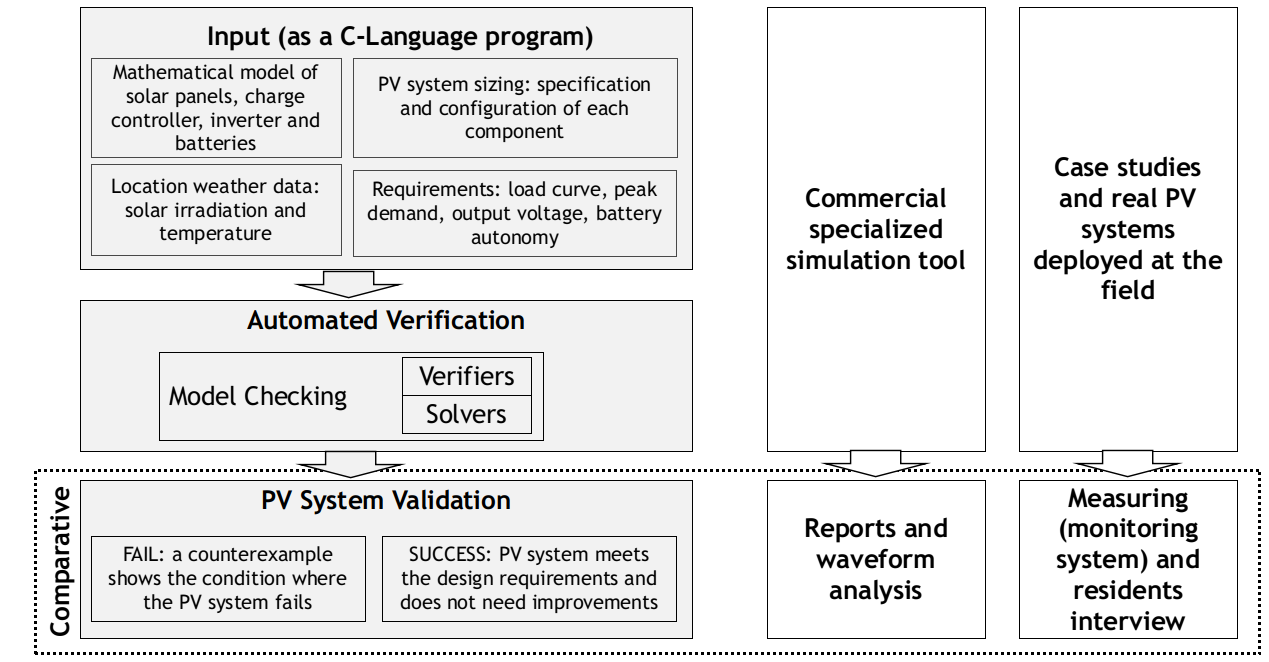
\includegraphics[width=0.85\textwidth]{verification_outline3.png}
\centering
\caption{Proposed validation of PV systems via automated verification.}
\label{fig:validation_outline} 
\end{figure}


\begin{figure}[h]
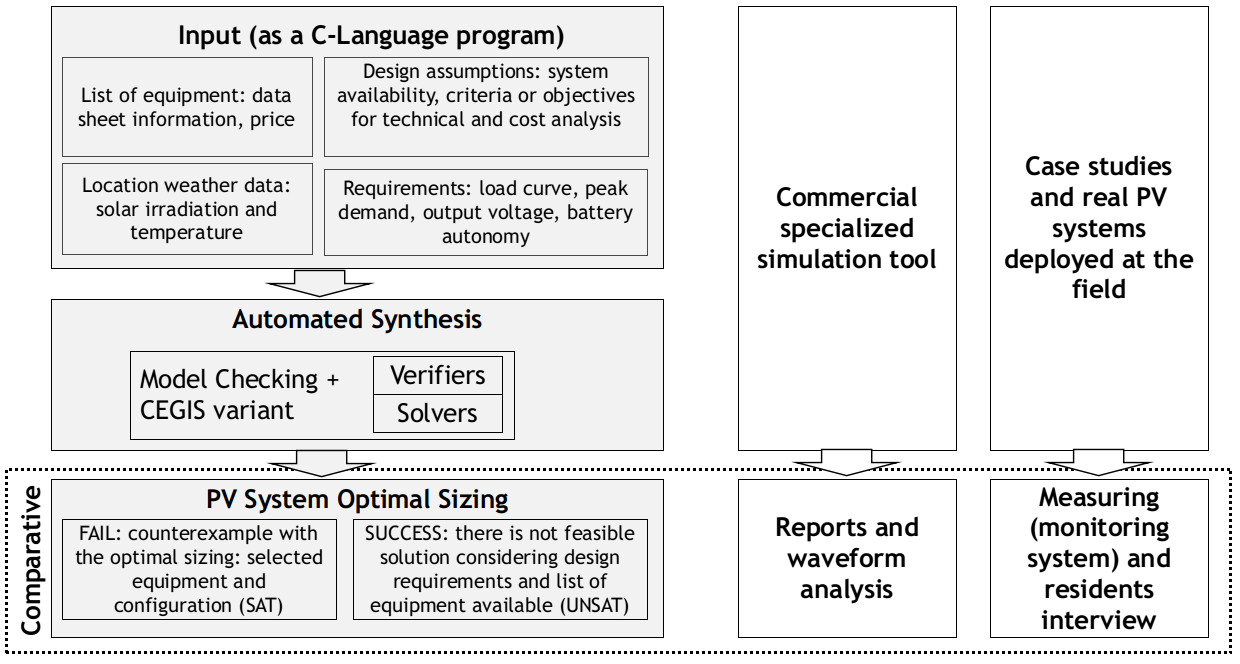
\includegraphics[width=0.85\textwidth]{optimization_outline3.png}
\centering
\caption{Proposed optimal sizing of PV systems via automated synthesis.}
\label{fig:optimization_outline} 
\end{figure}

Note that it is out of our scope to perform code modification on the verifiers or the solvers used during the automated verification or automated synthesis steps of our approach. Here we intend to create front-end applications for the verifiers and solvers (which are the back-end). That decision is based on the fact that we can be verifier-independent, and evaluate different back-ends, now and in the future, always searching for the best performance and soundness.

%----------------------------------------------
\section{Contributions}
%----------------------------------------------

With respect to the proposed \textbf{automated verification} technique, this thesis makes three main contributions: \textbf{first}, we propose an algorithm written in the C programming language which implements the automated verification method to formally check the sizing and the operation of a given stand-alone PV system; \textbf{second}, we evaluate the verification technique by comparing three state-of-the-art model checkers in five real case studies; \textbf{third}, experimental results show that this approach can find subtle design errors in stand-alone PV systems not easily detected by other approaches based on simulation.

In the area of \textbf{automated synthesis}, our study makes a further three original contributions: \textbf{first}, it is the first application of a sound and automated formal synthesis approach which can provide accurate results for optimal sizing of stand-alone PV systems; \textbf{second}, we propose a variant CEGIS method of synthesis with striking differences of how the Synthesize and Verify phases from the original CEGIS work (without solution candidate vector and using an incremental and iterative loop to reach the optimal cost solution); and \textbf{third}, experimental results in seven case studies show that our approach qualitatively outperforms state-of-the-art simulation tools: our solution is far more detailed and closer to real PV systems than solutions presented by simulation.
% Firstly, we describe a modular modeling of each component of a PV system by means of mathematical models that can be encoded into fragments of first-order theories supported by software model checkers. Secondly
%
%With respect to the proposed \textbf{automated verification} method, this thesis makes three main contributions. 
%\textbf{First}, we propose an algorithm written in the C programming language, which implements the automated verification method to formally check the sizing and the operation of a given stand-alone PV system. \textbf{Second}, we evaluate the verification method by comparing three state-of-the-art model checkers in five real case studies. \textbf{Third}, experimental results show that this proposed approach can find subtle design errors in stand-alone PV systems, which are not easily detected by other approaches based on simulation. 
%
%The framework provided at this paper outlines the requirements, the process and the mathematical modeling to perform automated formal verification of a stand-alone PV system, using the satisfiability modulo theories (SMT)-based verification method.
%
%And linked to \textbf{automated synthesis}, our work makes more three original contributions: \textbf{First}, it is the first application of a sound and automated formal synthesis approach, which can provide accurate results of optimal sizing of stand-alone PV systems; \textbf{Secondly}, we propose a variant CEGIS method of synthesis with striking differences of how the {\sc Synthesize} and {\sc Verify} phases from original CEGIS work (without solution candidate vector and using an incremental and iterative loop to reach the optimal cost solution); and \textbf{Thirdly}, experimental results with seven case studies show that our approach qualitatively outperforms state-of-the-art simulation tool: our solution is far detailed and closer to real PV systems than the solution presented by simulation.
%
%three major contributions. 
%\textbf{First}, the use of automated symbolic verification methods in electrical systems was uncommon in recent prior studies~\cite{abs-1811-09438}, and specifically their use in synthesizing optimal PV sizing is unprecedented. Here, a list of PV components (i.e., PV panels, charge controllers, inverters, and batteries) can be fed to the proposed synthesis method together with the user requirements and environment constraints, and the proposed synthesis algorithm based on symbolic model checking can find the optimal solution in technical and economical terms. 
%\textbf{Second}, we evaluate different state-of-art symbolic software verifiers with the goal of obtaining the best performance in the verification back-end for synthesizing optimal PV systems, thereby being the first work that performs this type of evaluation. 
%\textbf{Third}, the experimental results show that the proposed synthesis method is an effective and efficient approach on the pursuit of the optimal solution of PV systems using formal methods, which outperforms existing state-of-the-art simulation tool. As a result, this thesis marks the first application of a sound and automated formal synthesis approach able to provide accurate results of optimal sizing of stand-alone PV systems. Thus, this research considerably advances the state-of-the-art in applied energy over the last two decades with the goal of optimally designing PV systems.
 
%---------------------------------------------- 
\section{Related Work}
%----------------------------------------------

In this section we discuss only the use of formal methods in electrical systems in general since optimization of PV sizing is currently not obtained by formal methods or even program synthesis. %Here we discuss only the use of formal methods on electrical systems in general since currently there exists no use of it or even program synthesis to obtain the optimization of PV sizing.

The conversion of the traditional power grid into a smart grid, a fundamental example of a CPS, raises many issues that require novel methods and applications. In $2012$, a Chinese smart grid implementation was considered as a case study to address the verification problem for performance and energy consumption~\cite{Yukseletall2012}. The authors employed a stochastic model checking approach and presented a modeling and analysis study using PRISM, which is a probabilistic model checker~\cite{KwiatkowskaNP11}. The focus of this study was on how CPSs integrate information and communication technology functions to the physical elements of a system for monitoring and controlling purposes. The authors did not focus on power generation or even solar PV systems.

In $2015$, an automated approach for applying Monte-Carlo simulation to power system protection schemes presented limitations of incomplete coverage of all possible operating conditions~\cite{Sengupta2015}. The authors proposed an automated simulation-based verification technique to verify the correctness of protection settings efficiently using a hybrid automata-temporal-logic framework. The initial focus was on relay operations and test-case generation to ensure the early detection of design errors. However, this study was limited to power system protection and did not deal with electricity generation or even solar PV systems.

Other related studies from $2015$ include a framework named Modana to achieve an integrated process from modeling with SysML/MARTE to analysis using statistical model checking for CPS in terms of non-functional properties such as time and energy~\cite{Cheng2015}. In order to demonstrate Modana's capability, the authors modeled energy-aware buildings as a case study and discussed the analysis of energy consumption in different scenarios. The focus here is on smart buildings and HVAC (heating, ventilation, and air conditioning) systems. This research, however, did not address the design and verification of solar PV systems. 
 
In $2017$, a researcher suggested the application of formal methods to verify and control the behavior of computational devices, interacting over a shared and smart infrastructure~\cite{Abate2017}. The author discussed the aggregation of large populations of thermostatically-controlled loads and PV panels, and the similar problems of energy management in smart buildings, of demand-response on smart grids, and respectively of frequency stabilization and grid robustness. The focus was on controlling the behavior of components, thereby verifying the given smart grid as a ``system of systems'' within the context of "internet of things". The author, however, used an approximate model checking of stochastic and hybrid models.

In $2018$, a verification methodology was proposed for the Cyber-Physical Energy Systems (CPES) with applications to PV panels and its distributed powerpoint tracking~\cite{Driouich2018}. This approach relied on representing the unpredictable behavior of the environment to cover all possible feasible scenarios. The simulation results obtained by JModelica covered the system's complete dynamic behavior; however, almost three days of computer effort to verify the design space of a single operational hour of the PV panels’ behavior made it clear that time was an issue. This related study did not include any  other components of a stand-alone solar PV system. %however, it was evident the time-consuming issue with almost three days of computer effort to verify the design space of one operation hour of the PV panels behavior. This related study did not include other components of a stand-alone solar PV system.

Another study from $2018$ presented an approach to modeling smart grid components using a formal specification. The authors used a state-based formal specification language named Z; they demonstrated the application of Z to four smart grid components~\cite{Akram2018}. The formal specification presented can be considered a first step towards modeling smart grids using formal methods. The starting point of this study was that a smart home can be considered an integrated system consisting of various objects and systems, which communicate and interact with each other. This approach is based on Petri nets and works under the assumption that modeling smart homes leads to a clear understanding of the overall behavior of the smart grids.

However, prior studies did not deal with formal verification of a complete stand-alone PV system (with batteries, charge controller, and power inverter) or even solar PV systems optimization. Formal methods based on \textit{symbolic model checking} and its application to synthesize PV systems are still unexplored in the literature. Moreover, it is precisely on these gaps that this thesis is focused.

%----------------------------------------------
\section{Thesis Organization}
%----------------------------------------------

This introduction has outlined the context, motivation, and problem addressed by this thesis and the objectives, solution, and contributions of the research. The remaining chapters are organized as follows:

Chapter '~\nameref{chap:background}' presents the theoretical basis of formal methods, formal verification, automated verification, solar PV systems, design and validation of PV systems, program synthesis, and the mathematical modeling. 

Chapter '~\nameref{chap:automatedverification}' presents the automated formal verification technique, the experimentation details, and the results obtained with the tool created using this new method of PV systems validation. 

Chapter '~\nameref{chap:automatedsynthesis}' presents the automated synthesis technique from computer science and its application to obtain the optimal sizing of stand-alone solar PV systems, with details of the experimentation, and the results using the tools created to compare this new technique with a  simulation tool and from data collected from fieldwork. 

In the '~\nameref{chap:conclusions}' we present the main contributions, future work directions and concluding remarks.

~\autoref{chap:publications} presents a list of papers that we submitted to international journals and conferences on the topic of the automated verification method. It covers the years 2015-2019, restricted to the Ph.D. process.

~\autoref{chap:tools} depicts the tools created during the Ph.D process to implement and validate the two scientific methods of the thesis (and instructions for their use).

It is worth mentioning that we decided, with the consent of the coordination of the graduate program, that this document would be written in the active voice and entirely in English. The choice of the active voice comes from the choice of the English language, which in the thesis studied was always presented in the active voice. The decision to use the English language stems from the possibility that the research may lead to further developments and activities,  in the possibility of reaching a larger number of people and helping in the internationalization of the Federal University of Amazonas.